\section{互信息的辨别下界}
\label{sec:info-infonce}

上一节用互信息的上界推出辨别错误的下界。这一节方向相反：互信息本身难以计算时，用一个辨别问题做得有多好，给出互信息的下界。

互信息需要联合分布与边缘乘积的密度比$r=\mathrm{d}P_{X,Y}/\mathrm{d}(P_X\otimes P_Y)$，再对它取对数积分。在高维连续空间里，$r$常常写不出来，积分也难以计算；但从$P_{X,Y}$抽取配对$(X,Y)$、从$P_Y$抽取单个$Y$往往很容易。于是考虑一个辅助问题：把一个真正与$X$配对的$Y$藏在一堆与$X$无关的候选中，让一个评分规则把它找出来。$X$与$Y$关联越强，真配对越容易被认出；找得好，就说明互信息至少有这么大。

\subsection{候选配对的构造}
\label{sec:info-infonce-construction}

设$X,Y$取值于标准Borel空间，联合分布$P_{X,Y}$，正则条件分布$P_{Y\mid X}$存在。固定候选数$N\geq2$，按下面的方式产生$(X,J,Y_1,\dots,Y_N)$：
\begin{enumerate}
  \item 抽取$X\sim P_X$，并独立地从$\{1,\dots,N\}$中均匀抽取隐藏位置$J$；
  \item 给定$X=x$、$J=j$，令$Y_j\sim P_{Y\mid X}(\cdot\mid x)$，其余$Y_k\sim P_Y$（$k\neq j$），这$N$个候选在给定$(X,J)$时相互独立。
\end{enumerate}
记观测为$W=(X,Y_1,\dots,Y_N)$，$J$不被观测。图~\ref{fig:info-infonce-construction}画出了$N=4$时的构造。

\begin{BookInlineFigure}
  \centering
  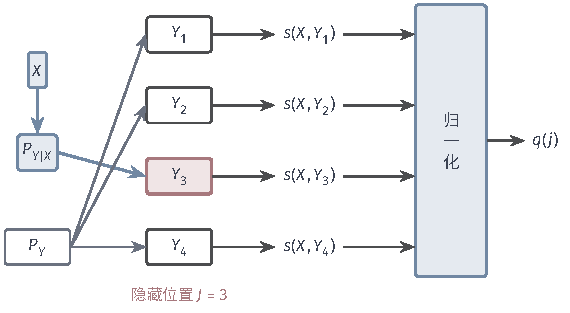
\includegraphics[width=96.4mm]{figures/07-probability/04-distribution-analysis/tikz/info-infonce-construction/figure.pdf}
  \caption{$N=4$个候选的构造。隐藏位置$J=3$（红框）的候选按给定$X$的条件分布$P_{Y\mid X}$产生（蓝），其余候选独立地按边缘分布$P_Y$产生（灰）。评分$s(X,Y_j)$经指数归一化得到对隐藏位置的猜测$q(j)$。}
  \label{fig:info-infonce-construction}
\end{BookInlineFigure}

这个构造有三条基本性质，后面的证明都靠它们。

\begin{lemma}[候选的分布]
\label{lem:info-infonce-structure}
在上述构造中：
\begin{enumerate}
  \item $J$与$X$独立；
  \item $(Y_1,\dots,Y_N)$独立同分布于$P_Y$，并且与$J$独立；
  \item 给定$J=j$，$(X,Y_j)$的分布是$P_{X,Y}$，其余候选独立同分布于$P_Y$，并与$(X,Y_j)$独立。
\end{enumerate}
\end{lemma}

\begin{proof}
第一条是构造的第一步。第三条：给定$J=j$，$X\sim P_X$且$Y_j$按$P_{Y\mid X}$产生，所以$(X,Y_j)\sim P_{X,Y}$；其余候选的条件分布不依赖$X$，所以与$(X,Y_j)$独立。第二条：在第三条中对$X$积分，$Y_j$的分布是$P_Y$，其余候选也是$P_Y$，且相互独立；这个分布不依赖$j$，所以候选组与$J$独立。
\end{proof}

第二条说明，单看候选组而不看$X$，完全看不出哪个是真配对；隐藏位置的线索只能来自$X$与各候选之间的关联。

\paragraph{隐藏位置的后验}
设$P_{X,Y}\ll P_X\otimes P_Y$，密度比为$r(x,y)$；$I(X;Y)<\infty$时这总成立。由引理~\ref{lem:info-infonce-structure}第三条，给定$J=j$时$W$的分布是$P_{X,Y_j}\otimes P_Y^{\otimes(N-1)}$，它相对于参考分布$P_X\otimes P_Y^{\otimes N}$的密度是$r(x,y_j)$。$J$的先验是$1/N$，由Bayes公式，
\begin{equation}
  \mathbb{P}(J=j\mid W)=\frac{r(X,Y_j)}{\sum_{k=1}^{N}r(X,Y_k)},\qquad j=1,\dots,N.
  \label{eq:info-infonce-posterior}
\end{equation}
分母几乎必然为正，因为真配对一项$r(X,Y_J)$几乎必然为正。后验只依赖各候选的密度比：与$X$越“般配”的候选，越可能是真配对。$X$与$Y$独立时$r\equiv1$，后验是均匀分布，候选无从区分。

\paragraph{二元例子}
仍用公平硬币$X$经以概率$\tfrac14$出错的线路得到$Y$。密度比在$y=x$时为$\tfrac{3/8}{1/4}=\tfrac32$，在$y\neq x$时为$\tfrac12$。取$N=2$。若两个候选相同（都等于$X$或都不等于$X$），后验是$(\tfrac12,\tfrac12)$；若只有一个等于$X$，由式~\eqref{eq:info-infonce-posterior}，它是真配对的后验概率为
\[
  \frac{3/2}{3/2+1/2}=\frac34.
\]
真配对等于$X$的概率是$\tfrac34$，另一个候选与$X$无关、是公平硬币，所以两个候选不同的概率恰为$\tfrac12$。

\subsection{InfoNCE下界}
\label{sec:info-infonce-bound}

实际中密度比$r$未知，用一个可测的实值\term{配对评分}（critic）函数$s(x,y)$代替$\ln r$，把评分作指数归一化得到对隐藏位置的猜测：
\begin{equation}
  q_s(j\mid W)=\frac{\mathrm{e}^{s(X,Y_j)}}{\sum_{k=1}^{N}\mathrm{e}^{s(X,Y_k)}}.
  \label{eq:info-infonce-softmax}
\end{equation}
用真实位置的平均负对数概率衡量猜得好坏，
\begin{equation}
  L(s)=\mathbb{E}\bigl[-\ln q_s(J\mid W)\bigr]\in[0,+\infty].
  \label{eq:info-infonce-loss}
\end{equation}
$L(s)$是真实后验相对于猜测$q_s$的交叉熵按$W$的平均。以$L$为目标的方法通称InfoNCE（信息噪声对比估计），它的总体值给出互信息的下界。

\begin{theorem}[InfoNCE下界]
\label{thm:info-infonce}
设$X,Y$取值于标准Borel空间，$I(X;Y)<\infty$，$N\geq2$，$s$是任意可测实值评分函数。则
\begin{equation}
  \ln N-L(s)\leq I(X;Y).
  \label{eq:info-infonce-bound}
\end{equation}
更精确地，
\begin{equation}
  I(X;Y)-\bigl(\ln N-L(s)\bigr)=I(X;Y_1,\dots,Y_N)+\mathbb{E}\Bigl[D_{\mathrm{KL}}\bigl(P_{J\mid W}\Vert q_s(\cdot\mid W)\bigr)\Bigr].
  \label{eq:info-infonce-gap}
\end{equation}
\end{theorem}

证明分三步：猜测的交叉熵不小于后验的熵；后验的熵等于$\ln N$减去隐藏位置与观测的互信息；这个互信息不超过原配对的互信息。

\begin{proof}
\emph{第一步。}固定$W=w$，$J$的后验$\pi(\cdot\mid w)$是$N$个点上的概率表。由定理~\ref{thm:info-cross-entropy-decomposition}（$N$点上的熵有限），
\[
  \mathbb{E}\bigl[-\ln q_s(J\mid W)\bigm|W=w\bigr]=H\bigl(\pi(\cdot\mid w)\bigr)+D_{\mathrm{KL}}\bigl(\pi(\cdot\mid w)\Vert q_s(\cdot\mid w)\bigr).
\]
对$W$平均，左端是$L(s)$，右端第一项是$H(J\mid W)$，于是
\[
  L(s)=H(J\mid W)+\mathbb{E}\bigl[D_{\mathrm{KL}}(P_{J\mid W}\Vert q_s(\cdot\mid W))\bigr]\geq H(J\mid W).
\]

\emph{第二步。}$J$均匀，$H(J)=\ln N$有限，由式~\eqref{eq:info-mi-entropy-difference}（对一般的$W$逐条件值进行），
\[
  H(J\mid W)=\ln N-I(J;W).
\]

\emph{第三步。}记$\bm{Y}=(Y_1,\dots,Y_N)$。用链式法则~\eqref{eq:info-mi-chain-rule}展开$I(J;W)=I(J;\bm{Y},X)$，由引理第二条$I(J;\bm{Y})=0$，所以
\[
  I(J;W)=I(J;X\mid\bm{Y}).
\]
另一方面，用两种顺序展开$I(X;J,\bm{Y})$。先$J$后$\bm{Y}$：由引理第一条$I(X;J)=0$；由引理第三条，给定$J=j$时只有$Y_j$与$X$相关，再用一次链式法则得$I(X;\bm{Y}\mid J)=I(X;Y)$。于是
\[
  I(X;J,\bm{Y})=I(X;Y).
\]
先$\bm{Y}$后$J$：
\[
  I(X;J,\bm{Y})=I(X;\bm{Y})+I(X;J\mid\bm{Y}).
\]
两式相等，而$I(X;Y)<\infty$，所以各项有限，可以移项，并由条件互信息的对称性得到
\[
  I(J;W)=I(X;J\mid\bm{Y})=I(X;Y)-I(X;\bm{Y}).
\]

三步合起来，
\[
  \ln N-L(s)=I(X;Y)-I(X;\bm{Y})-\mathbb{E}\bigl[D_{\mathrm{KL}}(P_{J\mid W}\Vert q_s)\bigr].
\]
这就是式~\eqref{eq:info-infonce-gap}；右端两个减项都非负，得到式~\eqref{eq:info-infonce-bound}。若$L(s)=+\infty$，式~\eqref{eq:info-infonce-bound}左端为$-\infty$，自然成立。
\end{proof}

式~\eqref{eq:info-infonce-gap}说明下界与真值之间有两段差距。第二段来自评分函数：只有$q_s$等于真实后验时才消失，由式~\eqref{eq:info-infonce-posterior}，这要求$s(x,y)=\ln r(x,y)+c(x)$，其中$c(x)$只依赖$x$（它在归一化中相消）。第一段$I(X;\bm{Y})$与评分无关，是辅助问题本身的损失：$X$与整组候选的互信息。它非负，所以即使评分最优，下界一般也严格小于$I(X;Y)$。

\paragraph{二元例子的计算}
取最优评分$s=\ln r$。$N=2$时，上一小节已得到：以概率$\tfrac12$两个候选相同，后验熵为$\ln2$；以概率$\tfrac12$两者不同，后验为$(\tfrac34,\tfrac14)$，熵为$h_{\mathrm{b}}(\tfrac14)$。于是
\[
  H(J\mid W)=\tfrac12\ln2+\tfrac12h_{\mathrm{b}}(\tfrac14)\approx0.3466+0.2812=0.6277.
\]
下界为
\[
  \ln2-L(\ln r)=\ln2-H(J\mid W)\approx0.0654,
\]
恰为$I(X;Y)\approx0.1308$的一半；由式~\eqref{eq:info-infonce-gap}，另一半是$I(X;\bm{Y})$。候选数增加时，计算方法相同：给定$X$，真配对以概率$\tfrac34$与$X$相同，其余$N-1$个候选各以概率$\tfrac12$与$X$相同，按相同候选的个数$m$求和，后验在相同者上为$\tfrac{3/2}{Z}$、在其余者上为$\tfrac{1/2}{Z}$，$Z=\tfrac32m+\tfrac12(N-m)$。

\begin{BookInlineFigure}
  \centering
  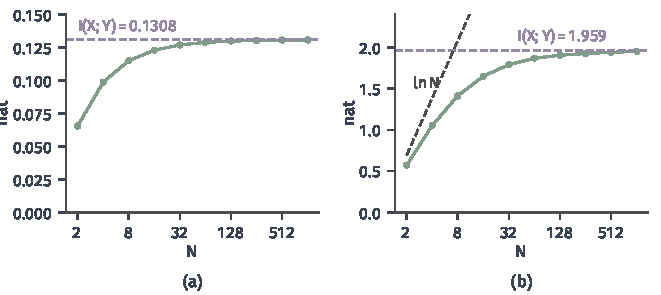
\includegraphics[width=112mm]{figures/07-probability/04-distribution-analysis/matplotlib/info-infonce-bound/figure.pdf}
  \caption{最优评分下的InfoNCE下界$\ln N-L$（绿）随候选数$N$的变化，横轴为对数刻度，紫虚线为$I(X;Y)$。(a)二元例子，按相同候选个数精确求和：$N=2,4,16,1024$时为$0.0654,0.0987,0.1229,0.1307$。(b)相关系数$0.99$的二元标准正态，$I(X;Y)\approx1.959$；Monte Carlo估计，种子$0$，每个$N$用$40000$组样本，标准误不超过$0.005$；灰虚线为$\ln N$。}
  \label{fig:info-infonce-bound}
\end{BookInlineFigure}

图~\ref{fig:info-infonce-bound}(a)中，下界随$N$增加逐渐逼近$I(X;Y)$：候选越多，$X$与整组候选的互信息在总量中所占的份额越小。这与“多个干扰项中认出真配对”的直觉一致，干扰项越多，认出真配对越能说明关联强。

\subsection{下界的限制}
\label{sec:info-infonce-limits}

\paragraph{候选数的上限}
$q_s\leq1$，所以$L(s)\geq0$，从而
\[
  \ln N-L(s)\leq\ln N.
\]
无论评分多好，下界都不超过$\ln N$。$I(X;Y)$很大时，要让下界接近它，候选数须达到$\mathrm{e}^{I(X;Y)}$的量级。图~\ref{fig:info-infonce-bound}(b)中相关系数为$0.99$的正态配对，$I(X;Y)\approx1.959$，$\mathrm{e}^{1.959}\approx7.1$；$N=2$时下界只有$0.57$，比$\ln2$略小，$N=8$时约$1.41$，直到$N$达到数百才接近真值。互信息每增加$1$ nat，所需候选数约乘以$\mathrm{e}$。

\paragraph{评分函数的限制}
评分函数通常只能从一个给定的函数类中选。在二元例子中限定$s(x,y)=c\,\mathbf{1}_{\{x=y\}}$，只调一个参数$c$。$N=2$时可以逐项算出$\ln2-L$：两个候选相同时$q$均匀；不同时真配对与$X$相同的概率是$\tfrac34$，被赋予$\mathrm{e}^{c}/(\mathrm{e}^{c}+1)$。于是
\[
  L(c)=\tfrac12\ln2+\tfrac12\Bigl[\tfrac34\ln(1+\mathrm{e}^{-c})+\tfrac14\ln(1+\mathrm{e}^{c})\Bigr].
\]
令导数为零得$\mathrm{e}^{c}=3$，$c=\ln3$正是$\ln\tfrac32-\ln\tfrac12$，这时评分等于$\ln r$加常数，下界达到$0.0654$。

\begin{BookInlineFigure}
  \centering
  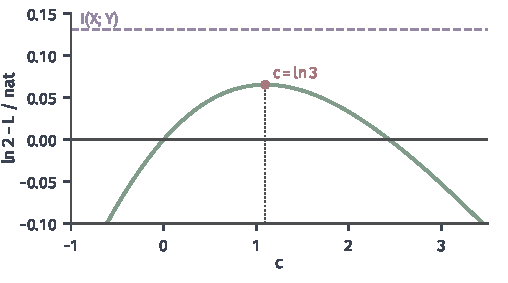
\includegraphics[width=86mm]{figures/07-probability/04-distribution-analysis/matplotlib/info-infonce-score/figure.pdf}
  \caption{二元例子、$N=2$、评分限定为$s(x,y)=c\,\mathbf{1}_{\{x=y\}}$时的$\ln2-L$（绿），紫虚线为$I(X;Y)\approx0.1308$。最大值在$c=\ln3$（红点）处，为$0.0654$；$c=0$时为$0$，$c=3$时约为$-0.053$。}
  \label{fig:info-infonce-score}
\end{BookInlineFigure}

图~\ref{fig:info-infonce-score}显示，$c=0$时评分不区分候选，下界为零；$c$过大时评分过于自信，猜错的代价很高，“下界”变成负数，仍然正确却毫无用处。一般的函数类不一定包含$\ln r+c(x)$，最优的$s$也只能逼近，式~\eqref{eq:info-infonce-gap}中的第二段差距一般不为零。

\paragraph{下界小不能推出独立}
由于上面两段差距，$\ln N-L(s)$接近零可能只是因为$N$太小、评分函数类太窄或选得不好。下界为零与$I(X;Y)=0$不是一回事；InfoNCE不是判断独立的判据，只是在已知互信息存在、需要其数值大小时提供的可计算下界。比较各种依赖度量能否刻画独立，是第~\ref{chap:dependence-measures}章的问题。

\paragraph{总体值与样本值}
定理~\ref{thm:info-infonce}中的$L(s)$是总体期望。实际计算时用一批样本的平均代替它，并且常用同一批样本挑选评分函数。样本平均有随机误差，可能高于真实的$L(s)$，也可能低于它；在同一批样本上挑出的评分，其样本平均系统性地偏低。所以单批样本得到的经验值并不自动是互信息的下界，图~\ref{fig:info-infonce-bound}(b)中的Monte Carlo值也只在标准误范围内可信。估计误差的控制与统计保证属于卷八的内容，可参考\BookChapterRef{chap:finite-sample-error-bounds}{卷八第4章“有限样本的误差上界”}。
